\documentclass[11pt]{article}

\usepackage{amsfonts}
\usepackage{amssymb}
\usepackage{amsmath}
\usepackage{epsfig}
\usepackage{hyperref}

\setlength{\textheight}{8.85in}
\setlength{\textwidth}{6.75in}
\setlength{\topmargin}{0.0in}
\setlength{\headheight}{0.0in}
\setlength{\headsep}{0.0in}
\setlength{\oddsidemargin}{-.125in}
\setlength{\parskip}{2mm}
\setlength{\parindent}{0mm}

%module 5 july 19, module 6 july 25
\begin{document}
\begin{center}
{\large \bf ACTSC 632 -- Project for Module 4 -- due on July 10} \\

\end{center}

This project will consider the German Credit data set available in the {\tt CASdatasets} package in which it is named {\tt credit}.  As a team of data analysts for a credit card company, you have been asked to compare different classification methods and provide a recommendation to your manager for which one is the best to identify the ``good'' (i.e., creditworthy, no non-payments) vs the ``bad'' (not credit-worthy, having existing non-payments) credit files.

This project is to be complete in teams. Information about teams' membership will be emailed on LEARN.

\begin{enumerate}
\item Determine the number of predictors in this data set, and whether they are quantitative of qualitative. How many observations are there? How many observations are classified as a ``bad credit''? ``good credit''?

  \noindent {\bf Solution:} There are 20 predictors, duration, credit\_amount, age are quantitative, and the other are qualitative. 
  Depending on the encoding used for the data set (which differs from source to source) the predictors  installment\_rate, residence\_since, existing\_credits and num\_dependents may be encoded as integers and thus be a priori be considered quantitative. But when looking at the meaning of the different values these predictors can take, it seems best to treat them as categorical. It won't matter in our analysis though, as these 4 predictors do not end up being considered in our models. and the others are categorical. %,  (althougare encoded as quantitative, the rest (13 of them) are categorical. 
  There are 300 observations out of 1000 classified as bad credit.
%\item Determine the value of $k$ to use in the KNN approach. Try three different values and argue which one should be retained for further analysis.
\item To explore the data further, produce the following plots: (i) for each of the predictors age and duration, make a box plot showing the distribution of the observations, separately for the ``good'' and ``bad'' observations.; (ii) for the pairs duration \& savings and duration \& credit history, plot the observations (using duration on the $x$ axis) and use different symbols for the ``good'' and ``bad'' observations. Comments on the plots you obtained.

  \noindent{\bf Solution:} For (i) we get

  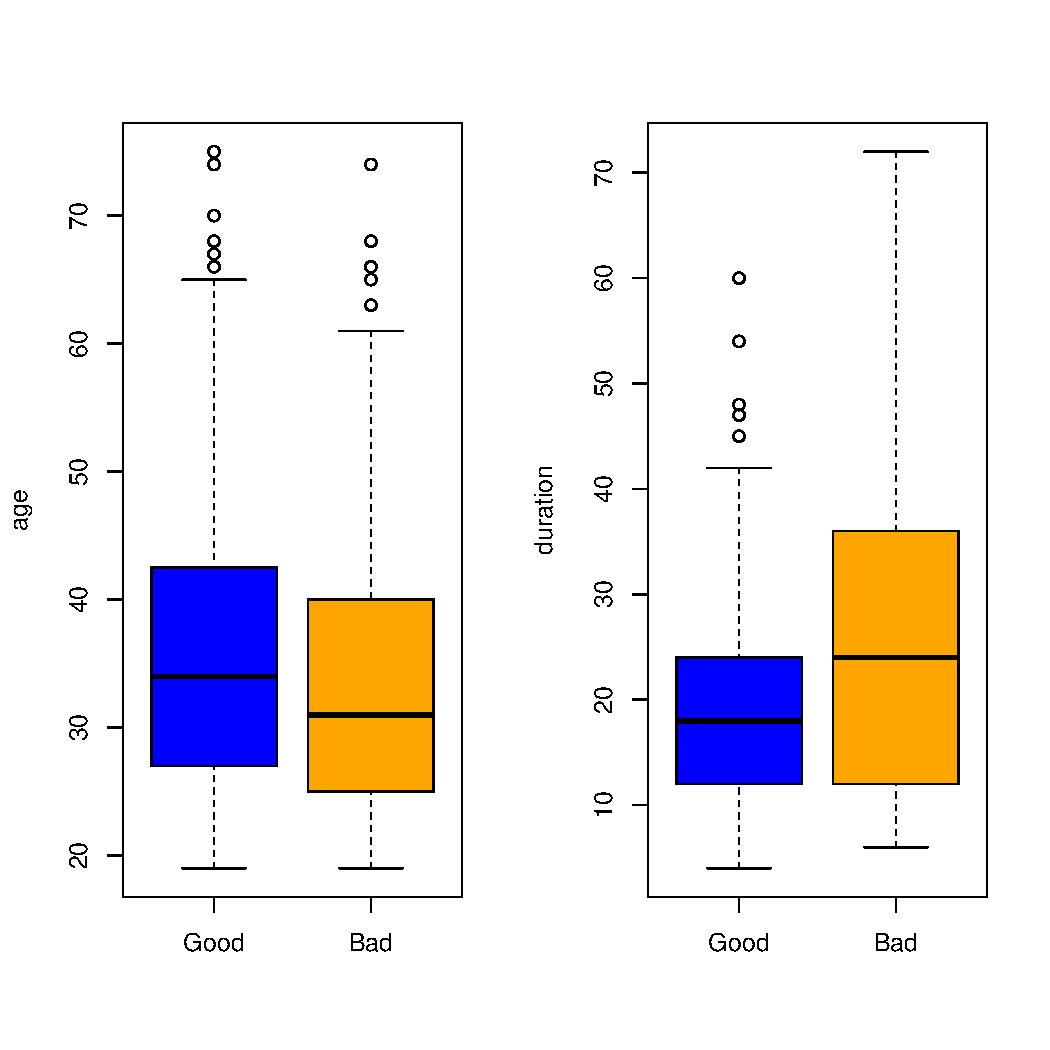
\includegraphics[scale=0.6]{box1.pdf}

  Clearly the bad credit observations seems to have a longer duration, and the distribution of the duration has a larger variance; they also seem to be slightly younger compared to the good credit.

  For (ii) we get
  \begin{figure}[htb]
  \caption{Bad credits shown in red, good shown in green}
  \begin{minipage}{0.48\linewidth}
  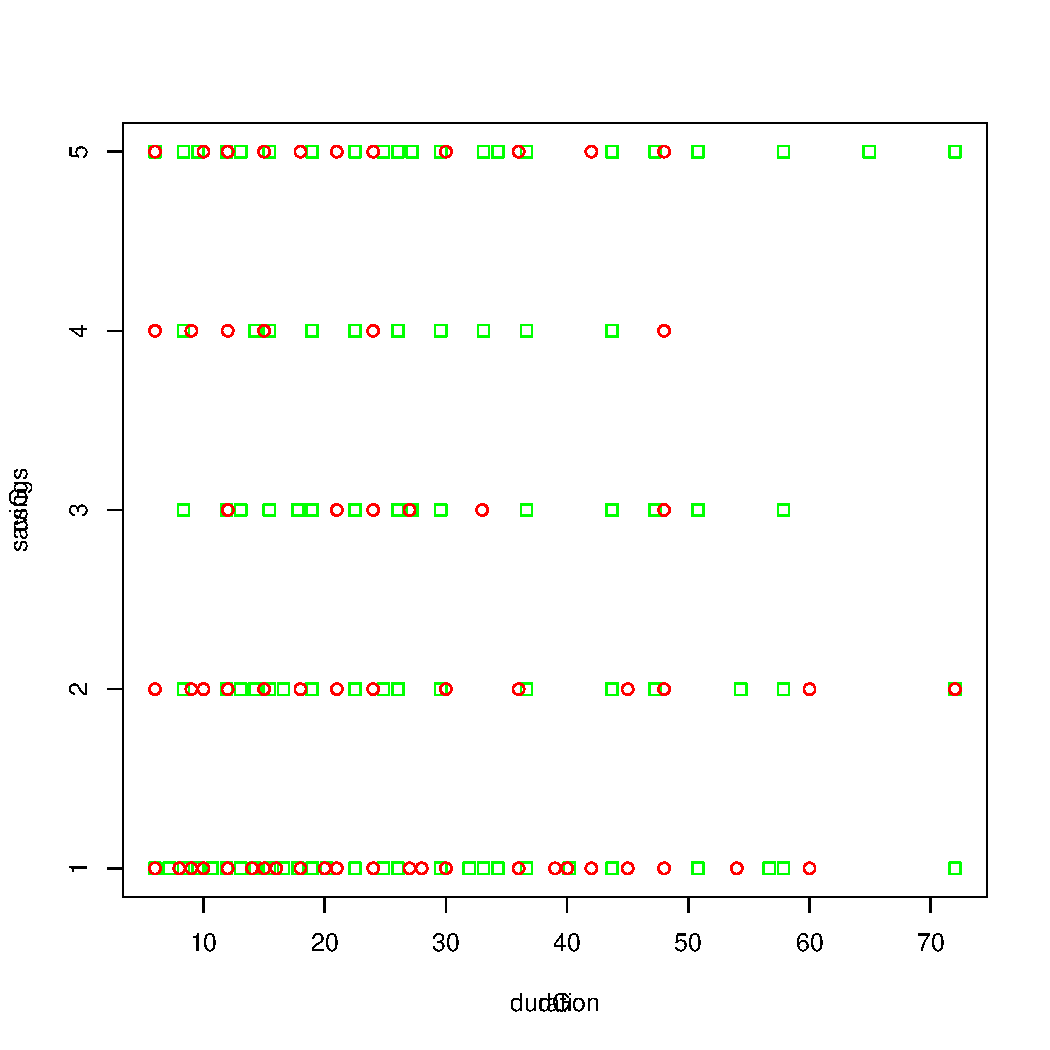
\includegraphics[scale=0.4]{dur-sav.pdf}
\end{minipage}
\begin{minipage}{0.48\linewidth}
  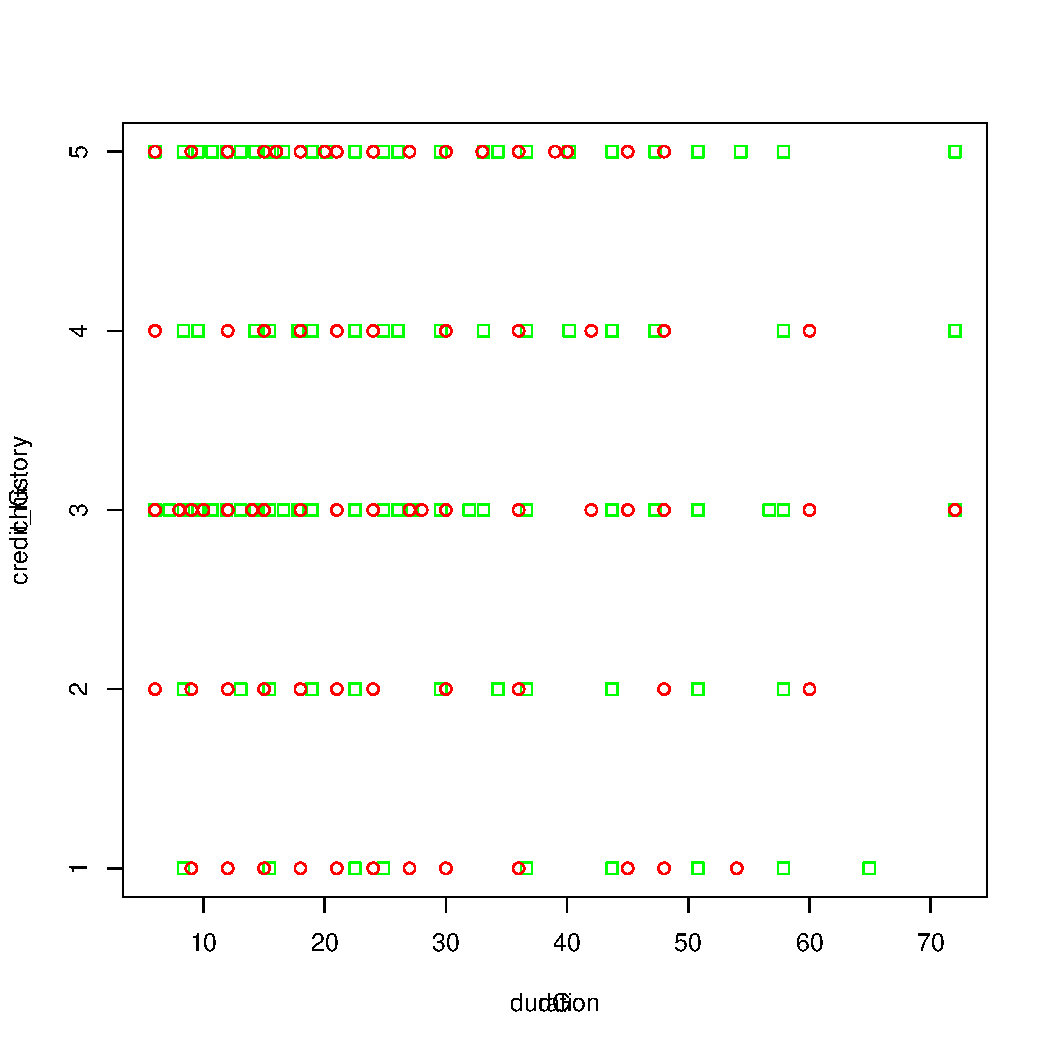
\includegraphics[scale=0.4]{dur-credh.pdf}
  \end{minipage}
  \end{figure}

  It is harder to see a clear trend in these two graphs, in that the good and bad credits are not easily classified according to duration for a given level of credit history or savings. Some observations on the duration vs savings plot is that most bad credits are on the lower values for savings (meaning they have less in their account) or in the 5th one, which means it is unknown whether or not they have a savings account. For the credit history
  
\item Initially, you should work with the following predictors: age, duration, purpose, credit\_history, and savings. For each of (i) logistic regression (ii) linear discriminant analysis (iii) quadratic discriminant analysis, do the following:
  \begin{enumerate}
  %\item Consider the age and duration predictor variables: plot the observations according to age (x axis) and duration (y axis) and then label them according to whether they are: TN, TP, FP, FN.
  \item Determine the confusion matrix, the overall error rate, Type-I error, Type-II error.

    \noindent{\bf Solution:} We get

    \begin{tabular}{| lll | lll |}
    \hline
   &&&overall&type 1& type 2\\   
    \hline
  logistic    &         0 &  1 &&&\\
  \hline
  0 &646& 192&&&\\
  1  & 54&  108&0.246&0.07714&0.64\\
  \hline
   lda    & 0&   1&&&\\
   \hline
  0 &644& 191&&&\\
  1 & 56& 109 &0.247&0.08&  0.6367\\
  \hline
qda    & 0 &  1 &&&\\
\hline
  0 &552& 133 &&&\\
  1 &148& 167 & 0.281 &0.2114 & 0.4433\\
  \hline
  \end{tabular}

    
  \item Plot the ROC curve for the three methods considered and determine the AUC (area under the curve).

    \noindent{\bf Solution:} the 3 ROC curves have respective AUC of 0.7609, 0.7613, 0.7461 and are given in Figure \ref{roc5pred}.

  \begin{figure}[htb]
  \caption{Logistic (left), lda  (right) and qda ROC curve (bottom) with 5 predictors}
  \label{roc5pred}
  \begin{minipage}{0.48\linewidth}
  \includegraphics[scale=0.4]{log4-roc.pdf}
\end{minipage}
\begin{minipage}{0.48\linewidth}
  \includegraphics[scale=0.4]{lda4-roc.pdf}
  \end{minipage}
  \centering
    \includegraphics[scale=0.4]{qda4-roc.pdf}
  \end{figure}

    
  \end{enumerate}
\item The manager who asked you to recommend a classifier for this problem says you'd be allowed to use up to two more predictors to build your classifier. Choose one or two additional predictors and determine how their inclusion affects the performance of the three classifiers (by repeating steps (a) and (b) in the previous question). Explain your choice of predictors.

  \noindent {\bf Solution:} We choose to add checking status and other parties after running a forward selection.

  We reran all three classifiers and got

\begin{center}
  \begin{tabular}{| lll | lll |}
  \hline
    & 0 & 1 & overall & type 1 & type 2 \\
    \hline
    logistic &&&&&\\
      0& 627& 159&&&\\
      1  & 73& 141& 0.232 & 0.1043 & 0.53 \\
      \hline
     lda     &  0&   1&&&\\
      0 &629& 152& & & \\
      1&  71& 148 & 0.223 &  0.1043 &  0.5067  \\
      \hline
 qda   & 0  & 1&&&\\
  0 &548&  93&&&\\
  1 &152& 207&0.245 & 0.2171 & 0.31 \\
\hline
    \end{tabular}
    \end{center}
    
  and the ROC curves  have respective AUC of 0.802, 0.8007, 0.7927 and are given in Figure \ref{fig:roc7}.



  \begin{figure}[htb]
  \caption{Logistic (left), lda  (right) and qda ROC curve (bottom) with 7 predictors}
  \label{fig:roc7}
  \label{roc5pred}
  \begin{minipage}{0.48\linewidth}
  \includegraphics[scale=0.4]{roc-log7.pdf}
\end{minipage}
\begin{minipage}{0.48\linewidth}
  \includegraphics[scale=0.4]{roc-lda7.pdf}
  \end{minipage}
  \centering
    \includegraphics[scale=0.4]{roc-qda7.pdf}
  \end{figure}
 
  
\item Suppose the credit card issuer assesses that it looses 4 times more money for each ``bad credit'' that is incorrectly identified (false negative)  as it does for a ``good credit'' that is incorrectly identified (false positive). Based on this, and using your results based on logistic regression with your choice of predictors from the previous question, propose a decision threshold  to identify a ``bad credit'' (via the estimated probability $\hat{P}(Y={\rm bad}|X)$) that minimizes the financial loss due to wrong classification. Then for all three methods, compute the overall (training) error rate, the type-I error and the type-II error. %For each of the three methods, identify on the ROC curve  the point that corresponds to this new threshold.

  \noindent{\bf Solution:} using logistic regression and the above cost function, we obtain a threshold of 0.167.

  We can re-run the prediction obtained from the three methods with this threshold and get

  \begin{tabular}{| l | lll |}
  \hline
   & overall & type-1 & type-2 \\
   \hline
    logistic &   0.359 & 0.4686 &0.1033\\
    lda&   0.356 &  0.4586 & 0.1167\\
    qda & 0.292 &0.3229 & 0.22\\
    \hline
  \end{tabular}
  
\item As an alternative to the previous question, suppose now that you wish to take a more conservative view point that does not rely on the above cost function, and instead what to choose the threshold that maximize Youden's J statistic (or equivalently, that maximizes the sum of the specificity and sensitivity). As in the previous question, compute the overall (training) error rate, the type-I error and the type-II error for all three methods using this new threshold. Comment on the results obtained using the three different thresholds used so far.

  \noindent {\bf Solution:} We find that the optimal threshold in that case is 0.295. We recompute the errors and get

     \begin{tabular}{| l | lll |}
  \hline
   & overall & type-1 & type-2 \\
   \hline
    logistic &   0.271 & 0.2786 & 0.2533\\
    lda&  0.277 &  0.2814 &  0.2667\\
    qda &  0.268 &  0.2714 & 0.26\\
    \hline
  \end{tabular}
  
  Overall, we see that using the threshold of 0.5 gives the lowest overall error, but find that for a small increase in the overall error, using the threshold of 0.295 that optimizes Youden's statistic provides a significant decrease in the type-2 error for logistic regression and LDA (going from  0.53 and 0.5067 to 0.253 and 0.267, respectively). The threshold of 0.167 provides the smallest type-2 error but at the expense of a large increase in the type-2 error.
  
  \item Using again what you believe is the best set of predictors from part 4, use $10$-fold cross-validation to estimate the overall error rate and  type-II error. Is it consistent with the training error rate?   Make sure to make your comparisons using the same threshold.

    \noindent {\bf Solution:} we use the threshold of 0.295 to answer this.  We use the function cv.glm (from the library boot) for logistic regression, and using the 0.295 threshold we get an overall error rate estimated to be 0.297 using 10-fold cv, and get 0.2776 for type-2 error. For lda we get 0.291 for the overall error rate and 0.2981 for the type-2 error. For qda, if we try all 7 covariates from part 4  we get an error of rank deficiency. Recall that both lda and qda are assuming all predictors are normally distributed, and as such when using these methods on data where some predictors are categorical, we are violating these assumptions and run the risk of having problems such as this one. I realize that some students determined it was not possible to answer this question for that reason and will not penalize them if they did so. Unfortunately I had not foreseen this problem when  preparing the assignment. If alerted to this earlier I would have suggested the following approach: remove problematic categorical predictor(s) to avoid the rank deficiency. After a few trials we see that removing ``purpose'' solves the problem. Using CV we get an estimated overall error of 0.29 and 0.3233. The corresponding error on the training sets are 0.263 and 0.2867.
    
    Hence in all three cases the training errors are slightly underestimated, as expected.
    

    
  \item Next you wish to use the $K$ nearest neighbours (KNN) as a classifier for this problem, using the three predictors age, duration and credit\_amount. Use a random sample of 750 observations as your training set and for each of $K=1,3,5$, apply the KNN approach. Produce the confusion table, determine the overall error rate, Type-I error and Type-II error. Which choice of $K$ seems the best?

    \noindent {\bf Solution:} we have used the 7 quantitative predictors and got

\begin{center}
    \begin{tabular}{| llll | lll |}
    \hline
      $K=1$&&0 & 1& overall & type-1 &type-2 \\
      \hline
            & 0& 132&  52&&&\\
            & 1&  30 & 36&0.436 &0.3631 &0.5909\\
      \hline
      $K=3$ &&0 &1&&&\\
      \hline
            & 0& 133&  55&&&\\
      & 1 & 29 & 33& 0.400 & 0.2043& 0.7045\\
      \hline
      $K=5$ &&0 &1&&&\\
      \hline
           & 0 &141 & 61&&&\\
      & 1 & 21 & 27& 0.364 &  0.1171 & 0.7614 \\
      \hline
    \end{tabular}
    \end{center}

    So from these results, choosing $K=5$ has the smallest prediction and type-1 errors, but $K=1$ has the smallest type-2 error.
    
  \item Now use 10-fold cross validation to estimate the overall error rate and Type-II error for each of $K=1,3,5$. Do you reach the same conclusion as in the previous question about the choice of $K$?

    \noindent {\bf Solution:} Using cv we get

    \begin{tabular}{llll}
      &$K=1$ & $K=3$ & $K=5$ \\
      \hline
overall&  0.385  & 0.348 &  0.342 \\
type-2 & 0.593 & 0.6767  & 0.76 \\
\hline
    \end{tabular}


    Based on the overall rate, using $K=5$ still seems the best choice.  The  error rates are consistent with what we obtained before.
    
  \item What would be your final recommendation for the best classifier to use for this problem?

    \noindent {\bf Solution:} Logistic regression would be my suggestion for this problem. It has good interpretative value compared to KNN, and unlike LDA and QDA, it doesn't rely on assumptions that are violated. The correspondng prediction errors are competitive with other methods.
\end{enumerate}

\end{document}
